\subsection{Gesamtkonzept}
\label{chap:grundkonzept}
\begin{figure}[h]
	\centering
	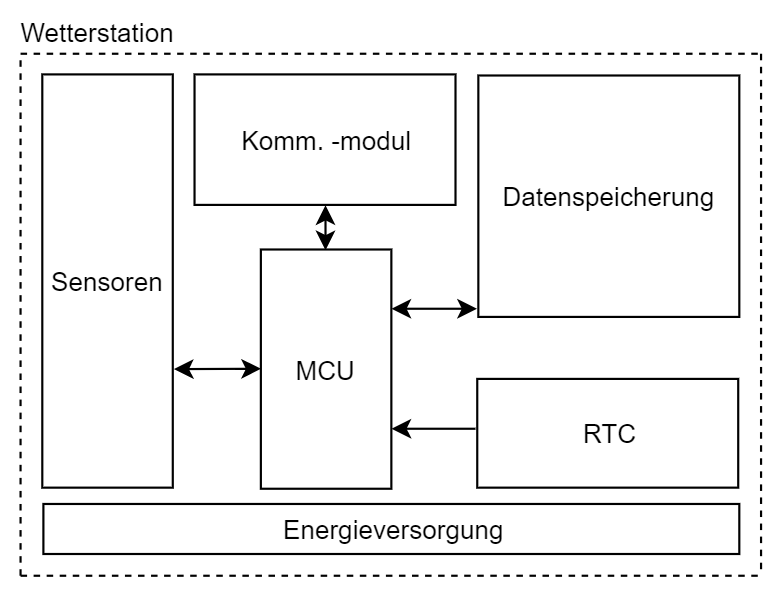
\includegraphics[width=0.9\textwidth]{graphics/Grundkonzept.PNG}
	\caption{Grundkonzept}
	\label{fig:grundkonzept}
\end{figure}

\paragraph{Übersicht:}
Als Zentralrecheneinheit wird eine \textit{Micro-Controller-Unit (MCU)} verwendet. Dieser ist dafür verantwortlich, dass die Daten richtig verarbeitet und an das dementsprechende Modul weitergeleitet werden. Die Messdaten werden in digitaler Form vom Modul \textit{Sensoren} an die \textit{MCU} übertragen. Dieser fügt mit dem \textit{Real-Time-Clock (RTC)} einen Timestamp hinzu, wobei anschließend die Daten in der \textit{Datenspeicherung} nichtflüchtig gespeichert werden. Über das \textit{Kommunikationsmodul} können dann die Daten von Nutznießern abgefragt werden.

Das Gesamtkonzept ist, wie in der Abbildung \ref{fig:grundkonzept} grafisch dargestellt, modular aufgebaut. Auf alle einzelnen Module wird folgend spezifischer eingegangen.\\
\newpage

\subsubsection{Micro Controller Unit (MCU)}
\begin{wrapfigure}{r}{0.5\textwidth}
  \vspace{-10pt}
  \begin{center}
    \missingfigure[figwidth=0.38\textwidth]{das Bild wird eh ersetzt oder sogar komplett gelöscht}
  \end{center}
  \vspace{-10pt}
  \caption{Arduino Mega \cite{Elektronik}}
  \vspace{-10pt}
  \label{fig:arduino_mega}
\end{wrapfigure}
Für die \textit{MCU} wurde im Projekt 5 ein Microcontroller mit bereits vorhandener Peripherie verwendet, welcher ähnlich wie der in Abbildung \ref{fig:arduino_mega} ersichtliche Arduino Mega aufgebaut ist. In diesem Projekt wird ein separates Printed Circuit Board (PCB) für die \textit{MCU} designed, welche die benötigte Peripherie aufweist. Auf diese Art kann Platz und Gewicht gespart werden, was der Mobilität der mobilen Wetterstation zugute kommt.\\

\subsubsection{Sensoren}
\begin{figure}[h]
\centering
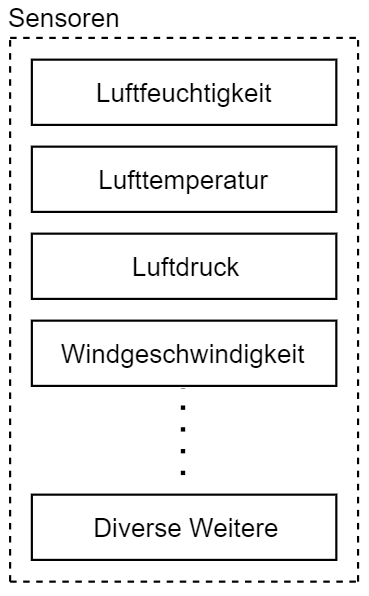
\includegraphics[scale=0.8]{graphics/Sensoren.PNG}
\caption{Sensoren}
\label{fig:sensoren}
\end{figure}
In dem Block \textit{Sensoren} werden alle Messeinheiten untergebracht. Die Idee dieses Blockes besteht darin, dass dieser adaptiv ist und somit leicht erweitert werden kann (Abbildung \ref{fig:sensoren}).\\
\todo[inline]{Inwiefern kann die Sensorik erweitert werden? Implementieren wir mehr Anschlüsse als gebraucht oder ist bloss die MCU erweiterbar mit einem zusätzlichen Print (aufsteckbar o.ä.)? -Erweiterungsmöglichkeit aufzeigen-}

\begin{figure}[h]
\centering
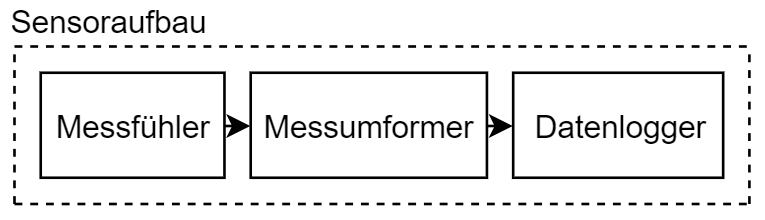
\includegraphics[scale=0.7]{graphics/Sensoraufbau.PNG}
\caption{Sensoraufbau}
\label{fig:sensoraufbau}
\end{figure}

\todo[inline]{Wird dieses Bild noch gebraucht?}

Im Projekt 5 wurde bereits die Sensorik zur Ermittlung der Lufttemperatur, Luftfeuchtigkeit, Luftdruck, Windgeschwindigkeit, Windrichtung und Regenmenge online erworben und implementiert. Im Projekt 6 wird die Sensorik zur Ermittlung der Sonnenstunden implementiert, sowie die gesamte Sensorik verifiziert und gegebenenfalls optimiert. Nachfolgend wird die Art und Weise erläutert, wie die Messdaten ermittelt werden.\\
\subparagraph{Windstärke:}
Die Windstärke wird über ein Schalenanemometer ermittelt. Mittels Reed-Kontakt wird die Drehfrequenz bestimmt und daraus eine Windstärkenstufe nach der Beaufort-Skala zugeordnet.\\
\subparagraph{Windrichtung:}
Die Windrichtung wird mit einer Windfahne gemessen, dessen Position mittels Reed-Kontakten ermittelt werden kann.\\
\subparagraph{Lufttemperatur, -Feuchtigkeit $\&$ -Druck:}
Die Lufttemperatur, Luftfeuchtigkeit und der Luftdruck werden über ein IC-Bauteil gemessen.\\
\todo[inline]{vellicht bitz detailierter?}
\subparagraph{Regenmenge:}
Für die Bestimmung der Regenmenge wurde auf eine alte aber effiziente Methode zurückgegriffen, das Kipplöffelprinzip. Bei diesem Prinzip füllt das Regenwasser einen Löffel der sich in der Ausgangsposition befindet, dieser Löffel kippt bei einer gewissen Menge und lässt einen zweiten Löffel in die Ausgangsposition heben. Über einen Reed-Kontakt wird die Kippfrequenz bestimmt, und daraus kann auf die Regenmenge zurück geschlossen werden.\\
\subparagraph{Sonnenstunden:}
Um die Sonnenstunden zu ermitteln, wird ein Sensor verwendet welcher die Bestrahlungsstärke misst. Die Sonnenstunden werden errechnet, wobei die Solarkonstante eine wichtige Rolle spielen dürfte.\\
\newpage
\subsubsection{Kommunikationsmodul}
\begin{figure}[h]
\centering
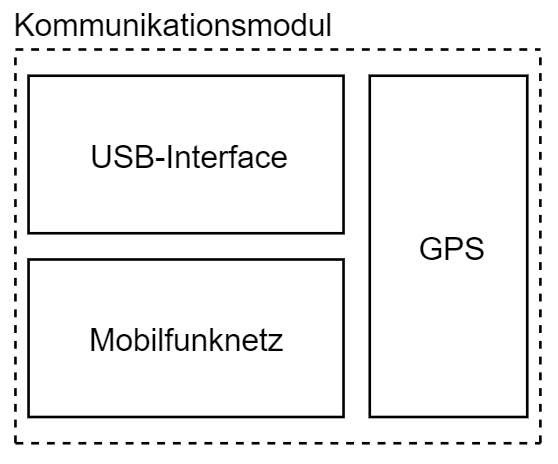
\includegraphics[scale=0.7]{graphics/Kommunikationsmodul.PNG}
\caption{Kommunikationsmodul}
\label{fig:kommunikationsmodul}
\end{figure}
Abbildung \ref{fig:kommunikationsmodul} zeigt die verschiedenen Schnittstellen, über welche Daten mit der Umgebung (User) und \textit{MCU} ausgetauscht werden können. Im Rahmen des Projekts 5 wurde das USB-Interface umgesetzt. Mobilfunknetz und GPS sind Teil des Projekts 6.\\

\subparagraph{USB-Interface:}
Über dieses Interface kann mit dem System kommuniziert und interagiert werden. Ein serielles Terminal-Emulationsprogramm (wie z.B. PuTTY) wird dazu benötigt.\\

\subparagraph{Mobilfunknetz:}
Die Einbindung der Wetterstation wird über diesen Block implementiert. Dazu wird ein GSM-Modul benötigt.\\

\subparagraph{GPS:}
Dieser Block sorgt für die Standortbestimmung. Dafür wird ein GPS-Modul auf dem PCB integriert.\\

\subsubsection{Datenspeicherung}
Die Datenspeicherung erfolgt auf einer $\mu$SD-Karte. Diese kann in ein Breakoutboard eingeschoben werden.\\
\todo[inline]{Stecke mer s Breakoutboard ufs PCB odr hesch du d circuits übernoh? Sunscht kurz aapasse dass es in e karteslot uf em pcb chunnt.}

\subsubsection{RTC}
Es wurde in einem vorhergehenden Projekt eine RTC implementiert, welche aktuelle Zeitstempel für erhobene Datensätze ermittelt.\\
\newpage
\subsubsection{Energieversorgung}
\begin{figure}[h]
\centering
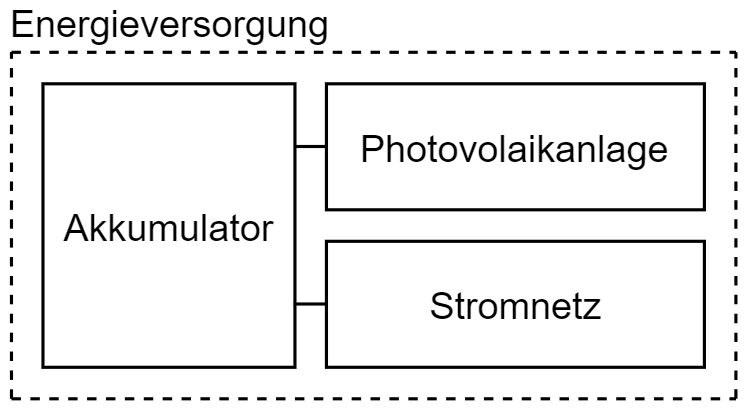
\includegraphics[scale=0.6]{graphics/Energieversorgung.PNG}
\caption{Energieversorgung}
\label{fig:Energieversorgung}
\end{figure}

Für die Speisung wird ein Akku verwendet. Gemäss Abbildung \ref{fig:Energieversorgung} soll dieser durch eine Photovoltaikanlage geladen werden. Als Wunschziel soll der Akku austauschbar sein.\\